%%% Document Author: J Moss
%%% Parts in LaTeX: Nicholas Dart
%%% Other Content: See authors list
%%% Document Last edit: 28.10.2014

\documentclass[11pt, article]{article}
\usepackage{a4wide}
\usepackage[english]{babel}
\usepackage{graphicx}
\usepackage{tabu}
\usepackage{textcomp}
\usepackage{fancyhdr}
\usepackage{lastpage}
\usepackage{titlesec}
\usepackage{lscape}
\usepackage{longtable}
\usepackage{fixltx2e}
\usepackage[T1]{fontenc}
\usepackage[toc,page]{appendix}

%%%%%%
%% Variables for version and release status
%% useage: \version
%%%%%%
\newcommand\module{CS21120}
\newcommand\moduleName{Program Design, Data Structures and Algorithms}
\newcommand\authorText{Nicholas Dart}
\newcommand\authorUsername{nid21}
\newcommand\studentID{130057750}
\newcommand\assesser{Bernie Tiddeman}

%%%%%%
%% Alias
%%%%%%
%%\newcommand{\sectionbreak}{\clearpage}    %% Allways start a section on a new page
%% Never worked anyway...
%% ]\newcommand{\figureRef[x]{i}{d}{l}}{\begin{figure} \centering \includegraphics[scale=x]{i} \caption{d} \label{fig:l} \end{figure}}

\title{ \huge \module Project \\ \Large \moduleName}
\author{
    \vspace{100pt}
    \begin{tabular}{ r || l }
        Author          & \authorText (\authorUsername)\\
                        & \studentID \\
        Date Published  & \today \\
                        & \\
        Assessed By     & \assesser \\
        Department      & Computer Science \\
        Address         & Aberystwyth University \\
                        & Penglais Campas \\
                        & Ceredigion \\
                        & SY23 3DB \\
    \end{tabular} \\
    Copyright \textcopyright Aberystwyth University 2014
    %get rid of the date on the titlepage
    \date{}
}

\pagestyle{fancy}
\fancyhf{}
\lhead{\module}
\rhead{\authorText  \studentID}
\rfoot{Page \thepage \hspace{1pt} of \pageref{LastPage}}
\lfoot{Aberystwyth University - Computer Science}

\begin{document}
    \centering
        \Large{\module: \moduleName}
    
    The task set forth in this assignemnt was to implement a program capable to be usable in a competition senario. It is to implement single and double elimination brackets.

    I made the assumption for double elimination that the loosers bracket is popped first, this is reflected in my unit tests.

    \newpage
    \begin{landscape}
            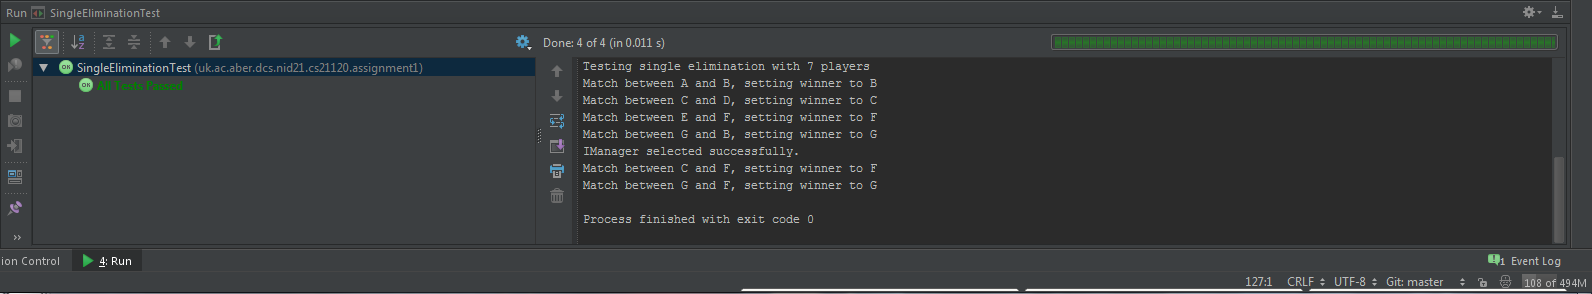
\includegraphics[scale=0.5]{singleElimination.png}\\
            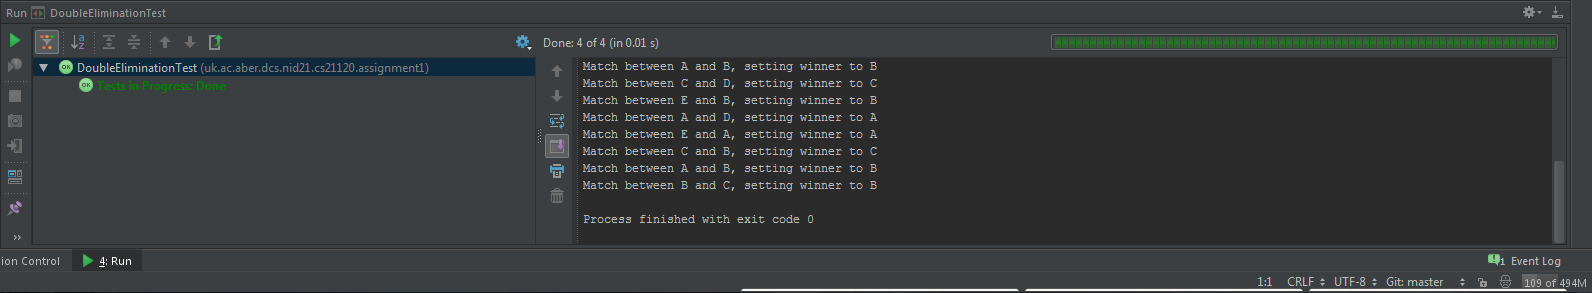
\includegraphics[scale=0.5]{doubleElimination.png}
    \end{landscape}

\end{document}